\documentclass[a4paper]{scrartcl}

%% Language and font encodings
\usepackage[english]{babel}
\usepackage[utf8x]{inputenc}
\usepackage[T1]{fontenc}

%% Sets page size and margins
\usepackage[a4paper,top=3cm,bottom=2cm,left=3cm,right=3cm,marginparwidth=1.75cm]{geometry}

%% Useful packages
\usepackage{amsmath}
\usepackage{graphicx}
\usepackage[colorinlistoftodos]{todonotes}
\usepackage[colorlinks=true, allcolors=blue]{hyperref}
\usepackage{placeins}
\usepackage{siunitx}
\usepackage{sidecap}
\usepackage{float}
\DeclareSIUnit\atmosphere{atm}

\title{Computational Motor Control - Lab 4}
\author{Florian Kaufmann \and Octave Martin \and Matthias Tsai}

\begin{document}
\maketitle

\section{Introduction}
The aim of this laboratory is to model central pattern generators to simulate a primitive behaviour of a lamprey neural system. By varying the parameters, we are going to experiment different simulations to help us understand the weight of each parameter and how to modify the behaviour of our lamprey model.

\section{Modelling the lamprey CPG with phase oscillators}
\subsection{Default parameters (6a.)}

We implemented a different chains of oscillators and varied the number of oscillators, the gradient of frequencies between them as well the coupling strength. To start of, we chose 10 oscillators, a frequency gradient of $\pi /6$ and a coupling strength of 7 to get an example of a phase locked chain of oscillators (see \cite{6astable}). From the plots, one can observe that the phase differences between the oscillators all stabilize to constant values and the oscillators visibly synchronize (left plot). Furthermore, despite of the intrinsic frequency gradient, the oscillators all agree on a common frequency during the simulation (right plot).

\begin{figure}[!h]
	\centering
	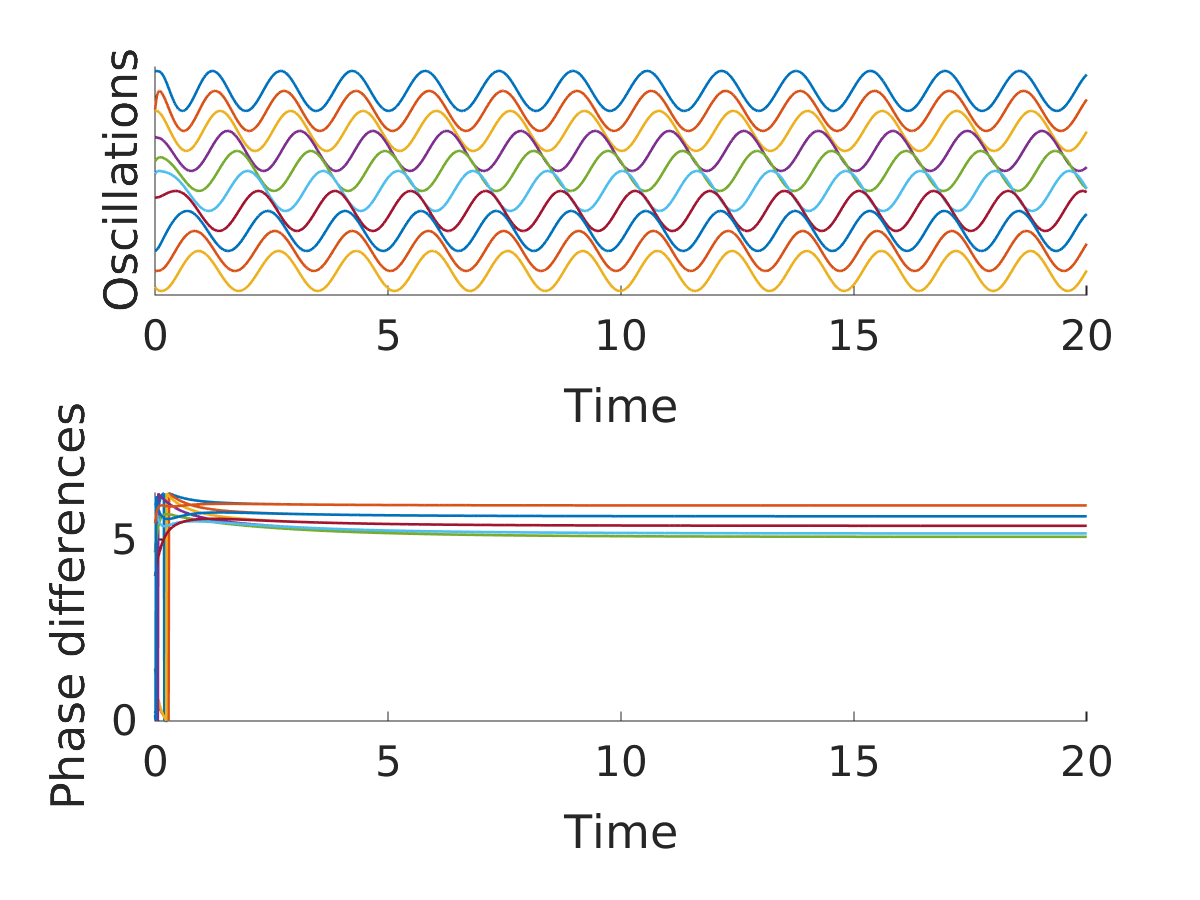
\includegraphics[width=0.5\textwidth]{fig/chain_phase_oscil-6a_stable.png}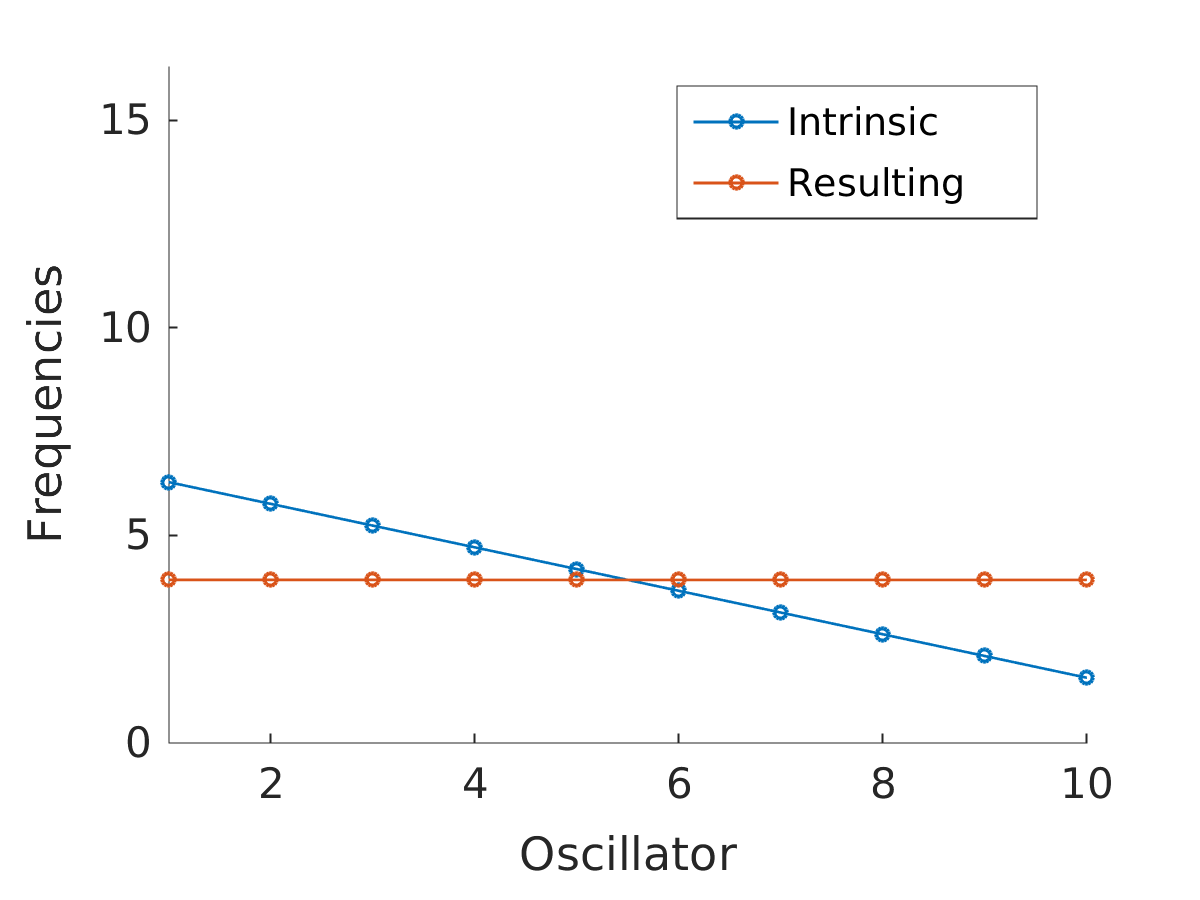
\includegraphics[width=0.5\textwidth]{fig/chain_phase_oscil_freq-6a_stable.png}
	\caption{Simulation of a chain of 10 phase oscillators with frequency gradient of $\pi /6$ and coupling strength of 7. Left: Oscillations and Phase differences of the oscillators over time.  Right: Plot of intrinsic frequencies and resulting frequencies from the simulation.}
\end{figure}

Next, we used our analytical formula to modify one parameter at a time to lose the phase locking behaviour of the chain of oscillators. First, the coupling strength was modified and reduced to 4 (see \cite{6aunstablecoupling}), and as predicted by our analytical prediction, the phase locking was lost. Interestingly, the chain of oscillators seems to have converged on two distinct frequencies, with the upper half of the chain synchronizing on a higher frequency as the lower part of the chain, with the central oscillators (especially the green one) experiencing quite some perturbation by being localized at the interface between these two subsystems.

\begin{figure}[!h]
	\centering
	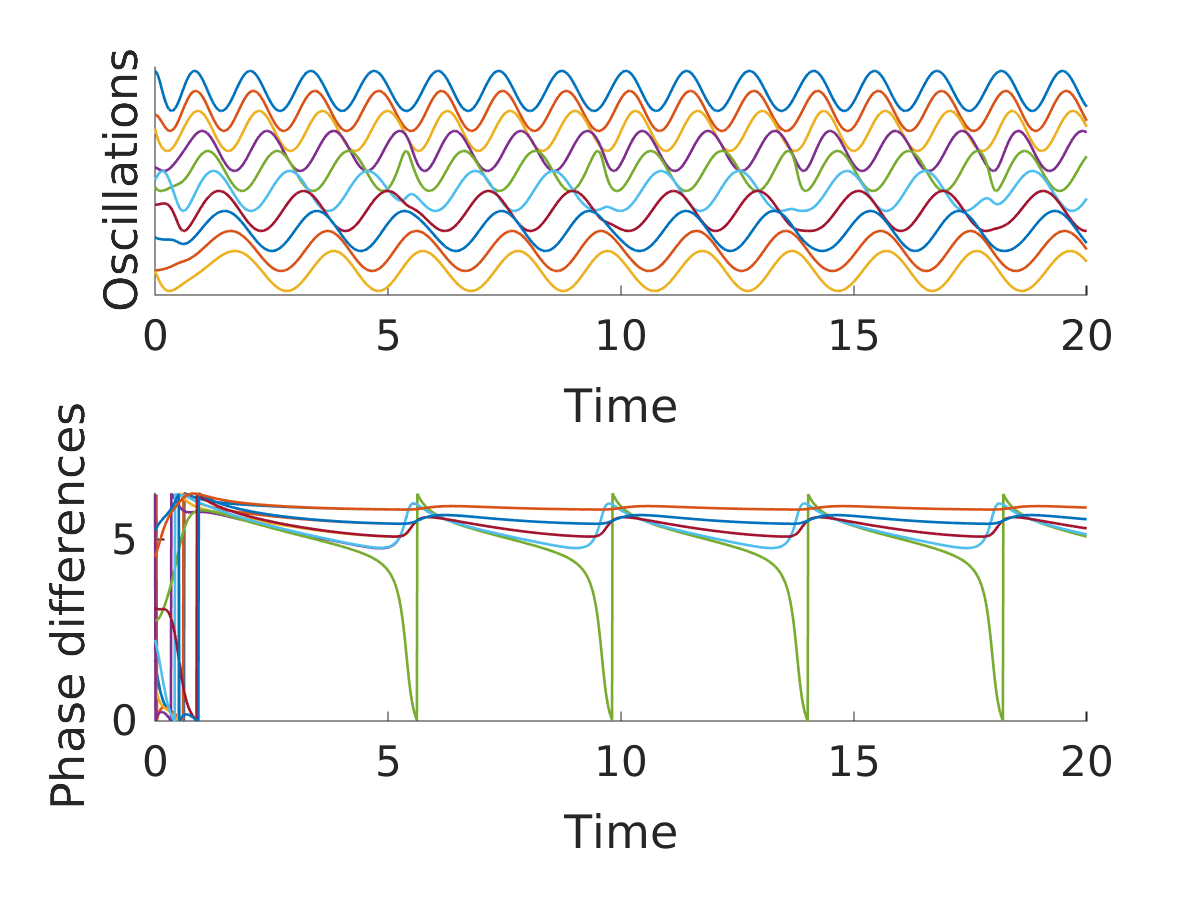
\includegraphics[width=0.5\textwidth]{fig/chain_phase_oscil-6a_unstable.png}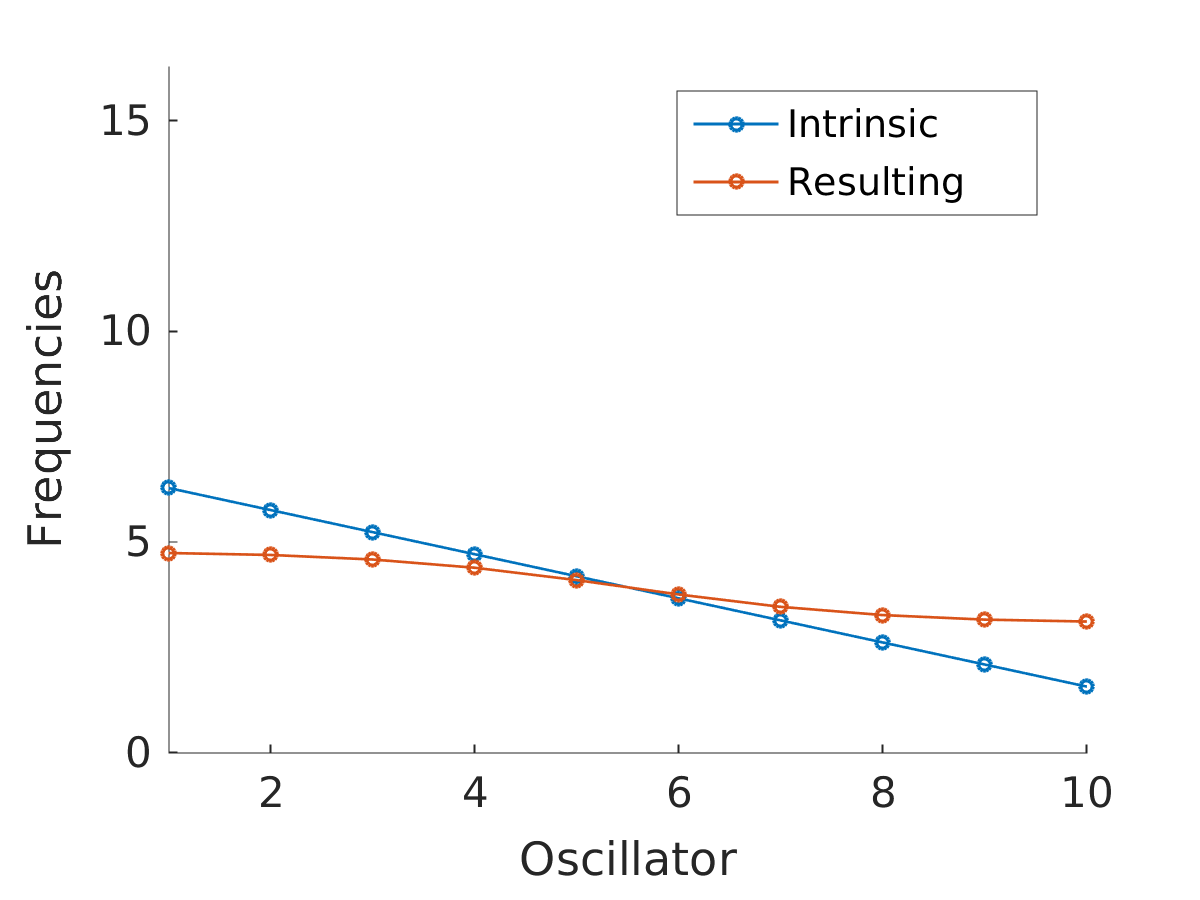
\includegraphics[width=0.5\textwidth]{fig/chain_phase_oscil_freq-6a_unstable.png}
	\caption{Simulation of a chain of 10 phase oscillators with frequency gradient of $\pi /6$ and coupling strength of 4. Left: Oscillations and Phase differences of the oscillators over time. Right: Plot of intrinsic frequencies and resulting frequencies from the simulation.}
\end{figure}

Similar loss of phase locking was also observed, if our initial phase locked oscillator chain was modified to either raise the frequency gradient to $\pi /5$ or to raise the number of oscillators to 11. This isn't very surprising, because by looking at the phase locking inequality condition using the parameters of our synchronized oscillator chain, one can predict that already a small change of one parameter in the wrong direction would change the sign of the inequality.

\begin{equation}
	coupling \_ strength = 7 > 6.545 =\frac{\pi \cdot 10^{2}}{6 \cdot 8} = \frac{frequency \_ gradient \cdot Noscils^2}{8}
\end{equation}


\newpage

\subsection{Possible non linear interesting model}

blabla

\newpage
\subsection{Influence of an external load}

blabla

\begin{figure}[!h]
	\centering
	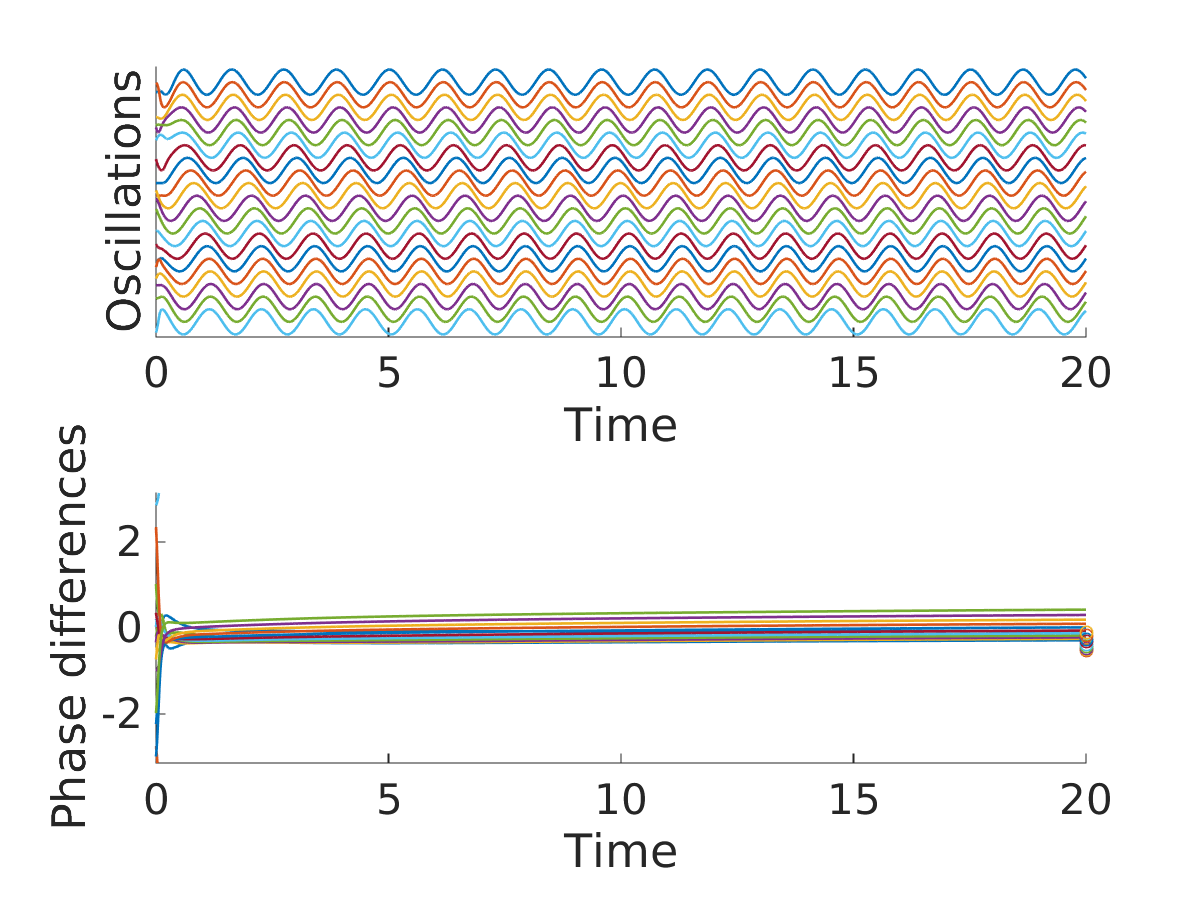
\includegraphics[width=0.5\textwidth]{fig/ext1.png}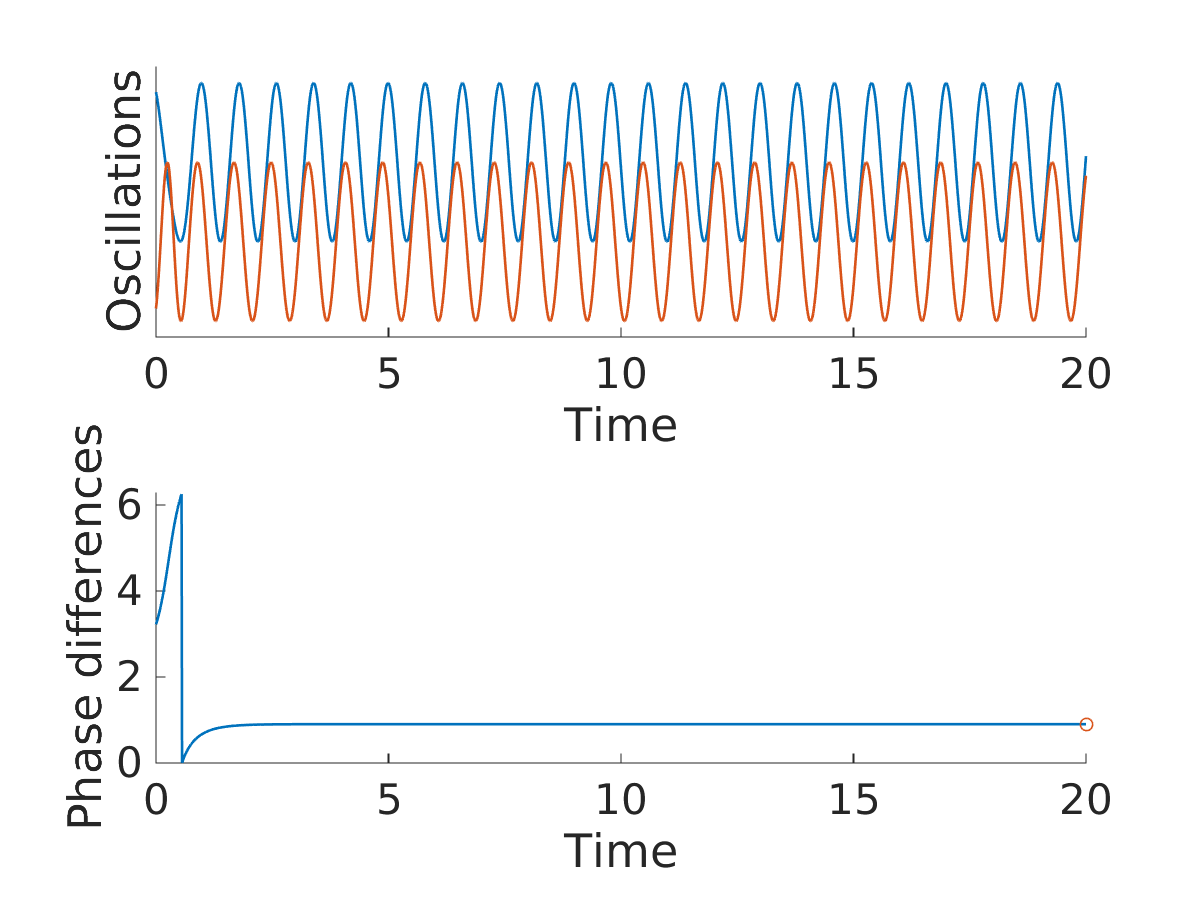
\includegraphics[width=0.5\textwidth]{fig/2phase.png}
\end{figure}

\begin{SCfigure}[][h]
	\centering
	\caption{ ... caption text ...}
	\includegraphics[width=0.5\textwidth]%
	{fig/ext3}% picture filename
\end{SCfigure}

\section{Comparing neuronal oscillators with phase oscillators}
\subsection{General behaviour (7.a)}

We saw  on the previous section that a phase oscillators with a good coupling has a smouth behaviour. A practical example could be 2 pendulums with an independant source of excitation coupled with a spring. If they have two intrinsic different frequency at the begining, there will be a transitory phase until they converge to the same freqency with some phase depending on the coupling strengh. The two signals in time look like sinusoidal curves. In opposition, for neuronal oscillators, it is possible to reach different modes of stable oscillations even with some crazy curves, see figure X.

\begin{figure}[!h]
	\centering
	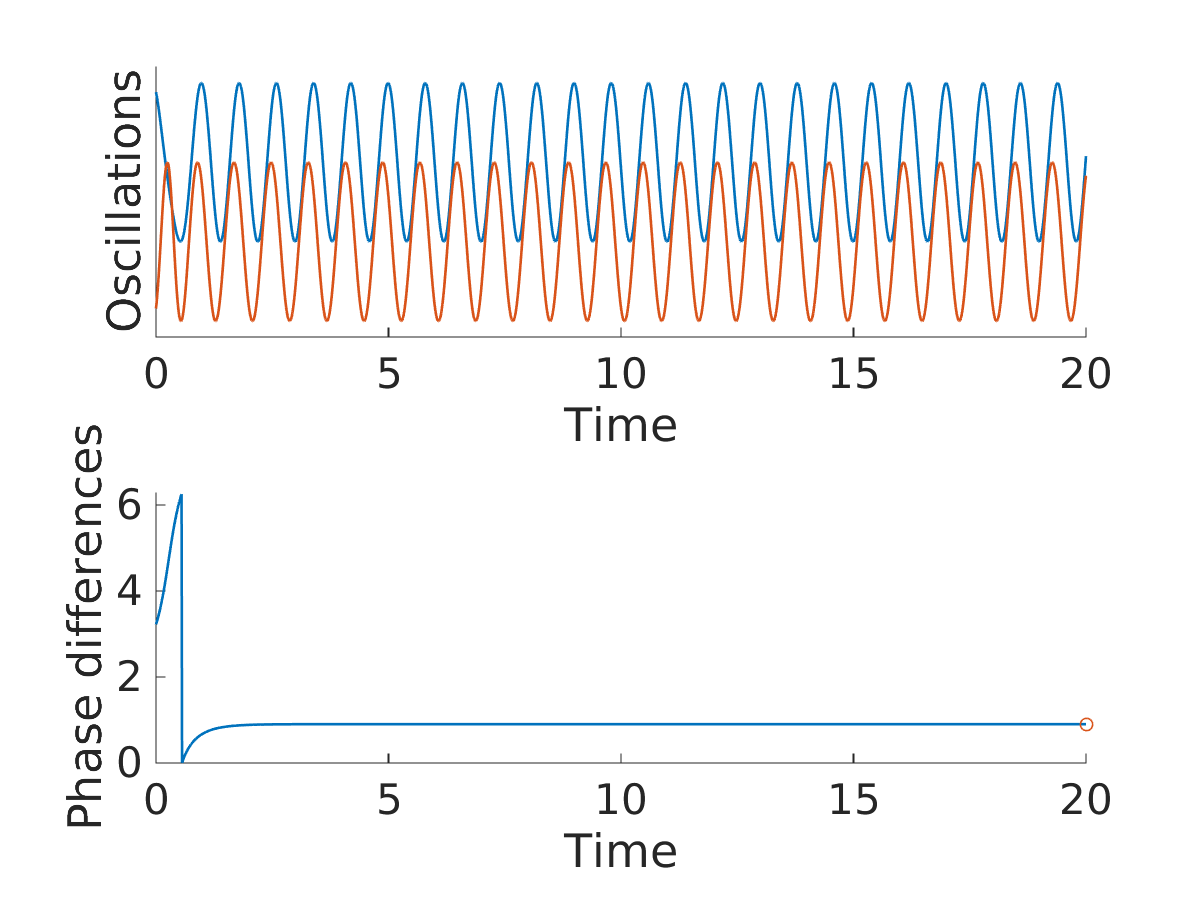
\includegraphics[width=0.5\textwidth]{fig/2phase.png}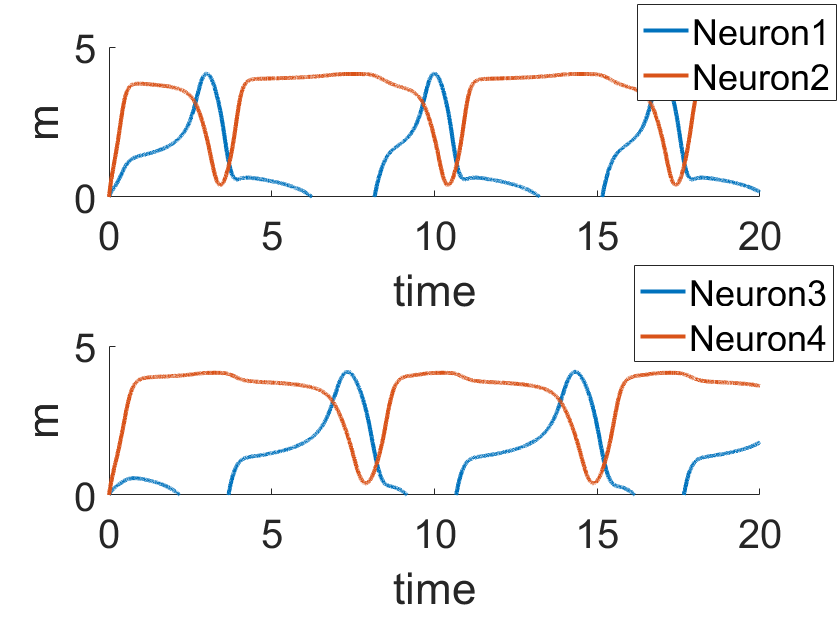
\includegraphics[width=0.5\textwidth]{fig/crazy.png}
	\caption{On the left picture, a stable phase oscillator and some crazy stable neuronal oscillations using a strong negative coupling on the right picture.}
\end{figure}

\newpage
When playing with the coupling strengh, one can observe two different behaviours. For the phase oscillators, a high coupling strengh results in the two masses oscillating at the same phase and frequency. If we add a strong positive coupling strengh to two neuronal oscillators, for example neuron 1 and 3, one can observe that the neurons will no longer oscillate but saturate to the maximum value because they excite one the other, see figure XX. The neurons 2 and 4 will be killed because of the negative feedback from neurons 1 and 2.

\begin{figure}[!h]
	\centering
	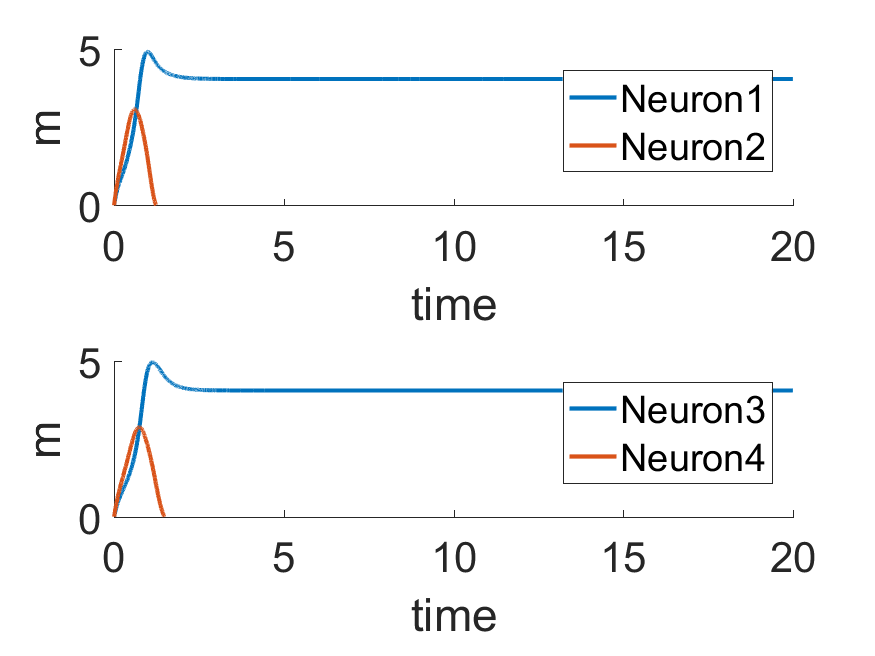
\includegraphics[width=0.5\textwidth]{fig/kill.png}
	\caption{Neurons with a high coupling strengh resulting in no oscillations.}
\end{figure}

\subsection{Comparing forced oscillators (7.b)}

If the periodic input is in the same range of frequency as the neuron 1, one can distinguish two extrem cases. Firstly, if the coupling strengh is low, the neuron 3 will lightly feel the influence of the input periodic signal, see fig (??)

\begin{figure}[!h]
	\centering
	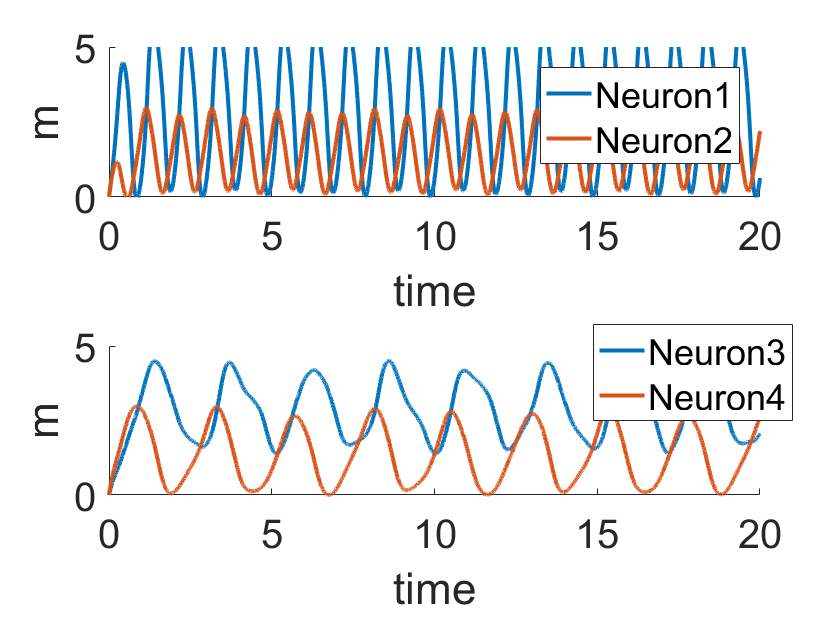
\includegraphics[width=0.5\textwidth]{fig/7b.png}
	\caption{Neuronal oscillators with a low coupling strengh and a periodic input on neuron 1.}
\end{figure}

\newpage

Secondly, one can observe that even if the neurons are overconstrained and then saturate, there will be a residual oscillations, see fig (!??). This is interesting to see because we can imagine that the environement dictate the coupling strengh and our neuronal system would oscillate in different modes depending one the coupling strengh between the neurons.

\begin{figure}[!h]
	\centering
	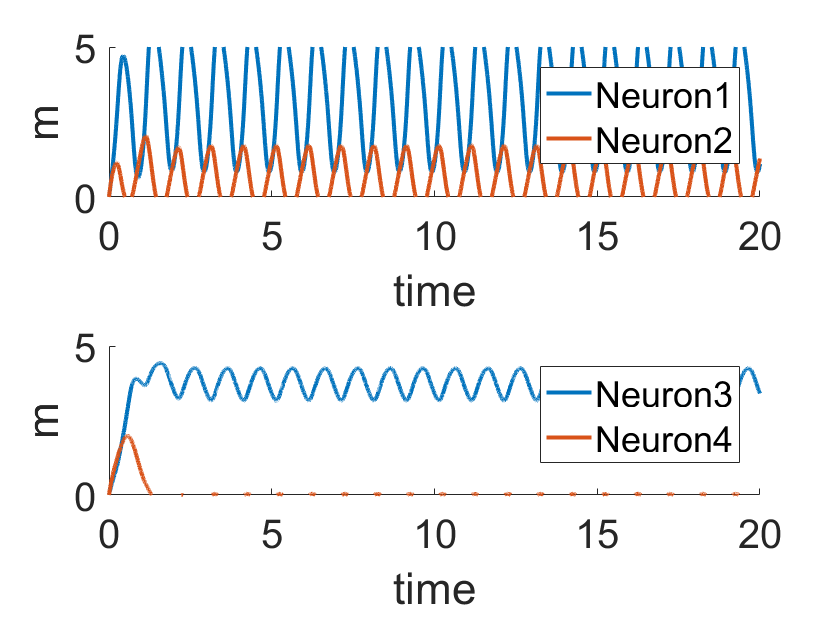
\includegraphics[width=0.5\textwidth]{fig/sat.png}
	\caption{A high coupling strengh on a neuronal oscillator excited by a periodic signal on the neuron 1.}
\end{figure}

In the case where the frequency of the input signal is way higher than the instrinsic frequency, ...

\newpage
\section{Conclusion}

blabla

\end{document}
